\section{Các phương pháp nén mô hình}
Over-parameterization là hiện tượng mạng tích chập chứa số lượng lớn neuron hoặc tham số không đóng góp đáng kể vào việc cải thiện độ chính xác. Các thành phần dư thừa này có thể được loại bỏ với mức suy giảm hiệu năng tối thiểu. Như minh họa trong Hình \ref{fig:my_optimization}, có ba hướng tiếp cận chính để tối ưu hóa mạng tích chập, bao gồm: thiết kế hoặc sinh tự động kiến trúc mạng,  thiết kế phần cứng chuyên biệt, và các kỹ thuật tối ưu bổ sung.
\begin{figure}[ht]
  \centering
  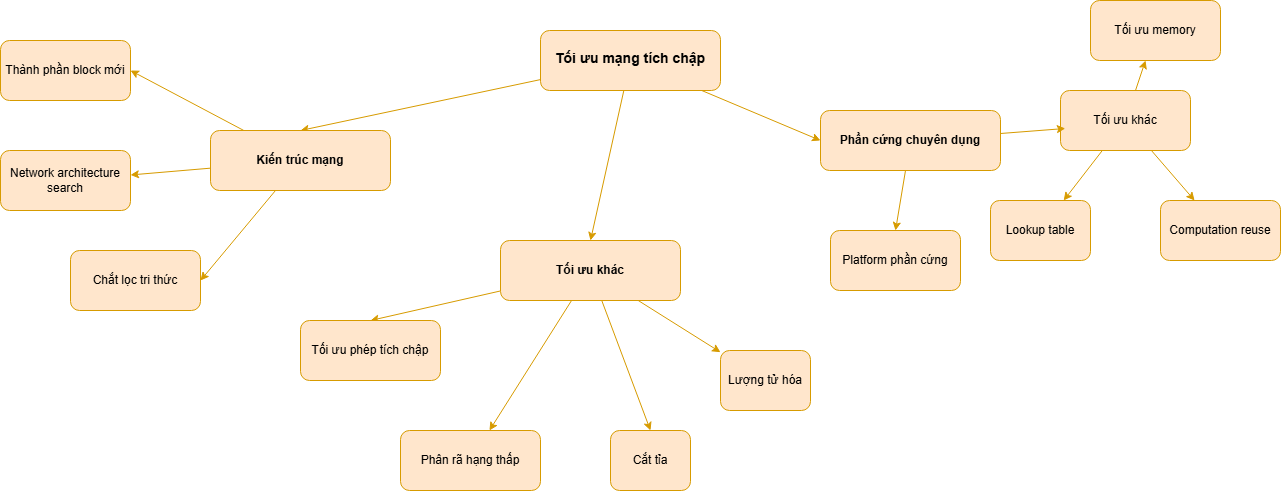
\includegraphics[width=\linewidth]{images/Optimization.drawio.png}
  \caption{Các phương pháp tối ưu hóa mạng tích chập}
  \label{fig:my_optimization}
\end{figure}
\subsection{Chắt lọc tri thức}
Chắt lọc tri thức (Knowledge Distillation – KD) là một kỹ thuật quan trọng trong nén mô hình, tập trung vào việc chuyển giao khả năng khái quát hóa từ một mô hình lớn hoặc một tập hợp các mô hình (gọi là teacher) sang một mô hình nhỏ hơn (gọi là student). Mục tiêu là duy trì hiệu suất của mô hình trong khi giảm đáng kể chi phí tính toán và yêu cầu bộ nhớ. Một framework KD điển hình thường bao gồm ba thành phần chính: dạng tri thức được chuyển giao, thuật toán chắt lọc, và kiến trúc teacher–student. Tổng quan của quy trình này thường được minh họa trong \ref{fig:KD_overview}.
\begin{figure}[ht]
  \centering
  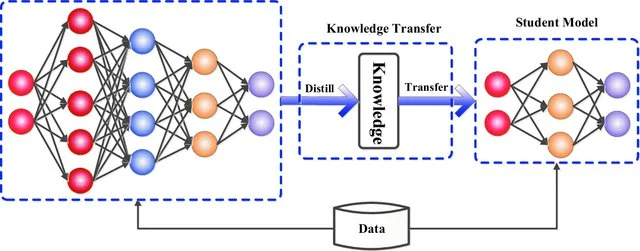
\includegraphics[width=\linewidth]{images/The-generic-teacher-student-framework-for-knowledge-distillation_W640.png}
  \caption{Quy trình chắt lọc tri thức}
  \label{fig:KD_overview}
\end{figure}

Mặc dù ứng dụng phổ biến nhất của KD là trong nén mô hình, phương pháp này cũng đã được mở rộng sang nhiều bài toán khác như tăng cường dữ liệu (data augmentation), học đối kháng (adversarial learning), và học biểu diễn. Về mặt lịch sử, ý tưởng nền tảng của KD được đề xuất bởi Cristian Bucilă et al. (2006)\cite{KD_10.1145/1150402.1150464}, với mục tiêu chuyển giao tri thức từ mô hình phức tạp sang mô hình đơn giản hơn. Khái niệm Knowledge Distillation sau đó được chính thức hóa và phổ biến rộng rãi bởi Geoffrey Hinton và et al.(2015)\cite{46_Hinton2015DistillingTK}. Trong những năm gần đây, KD đã phát triển mạnh mẽ với nhiều biến thể khác nhau, mở rộng cả về phương pháp lẫn phạm vi ứng dụng.  

Dựa trên dạng tri thức được chuyển giao, Knowledge Distillation có thể được chia thành ba nhóm chính. Response-based Distillation tập trung vào đầu ra của mô hình giáo viên, với mục tiêu giúp mô hình học sinh mô phỏng phân phối xác suất của giáo viên thay vì chỉ học từ nhãn cứng. Trong bài toán phân loại, tri thức phổ biến nhất là soft targets của Hinton\cite{46_Hinton2015DistillingTK}, được tính bằng hàm softmax với nhiệt độ T:
    \begin{equation}
        p(z_{ij},T) = \frac{e^{\frac{z_{ij}}{T}}}{\sum_ke^{\frac{z_{ik}}{T}}}
    \end{equation}
với $z_{ij}$ là logit của lớp thứ j của mẫu i, và T là nhiệt độ điều khiển độ mềm của phân phối. Hàm mất mát chắt lọc thường được định nghĩa bằng Kullback Leibler divergence giữa teacher-student và trong thực tế, hàm mất tổng sẽ được kết hợp cùng với cross-entropy loss giữa student và ground-truth label: 
     \begin{equation}
     \begin{aligned}
          L_{ResD} &= KL(p_t^{(T)}||p_s^{(T)})\\
          &= \sum\limits_{i=0}^M\sum\limits_{j=0}^Np_t^{(T)}(z_{ij})log\left(\frac{p_t^{(T)}(z_{ij})}{p_s^{(T)}(z_{ij})}\right)
     \end{aligned}
     \end{equation}
     \begin{equation}
         L = \alpha L_{CE} + (1-\alpha)T^2L_{ResD}
     \end{equation}

Ngược lại, Feature-based Distillation khai thác biểu diễn trung gian (feature maps) của mô hình giáo viên để hướng dẫn mô hình học sinh. Hàm mất mát có dạng tổng quát như sau: 
    \begin{equation}
        L_{FeaD} = L_F(\phi_t(f_t(x)),\phi_s(f_s(x))
    \end{equation}
trong đó $f_t(x)$, $f_s(x)$ là feature maps của teacher và student, $\phi_t(.)$, $\phi_s(.)$ là hàm biến đổi dùng khi kích thước feature không khớp, $L_F$ là hàm đo độ tương đồng. 

Ngoài ra còn có Relation-based Distillation, trong đó giá trị feature không được học trực tiếp, mà thay vào đó là học mối quan hệ giữa các feature hoặc giữa các mẫu dữ liệu, giúp mô hình học sinh học được cấu trúc hình học của dữ liệu. Trong đó, hàm mất mát chắt lọc dựa trên quan hệ giữa các mẫu có dạng như sau:
        \begin{equation}
            L_{RelD} = L_R(\psi_t(f_t(x_i),f_t(x_j)),\psi_s(f_s(x_i),f_s(x_j))
        \end{equation}
trong đó $x_i$, $x_j$ là cặp dữ liệu đầu vào, $\psi_t(.)$, $\psi_s(.)$ là hàm đo độ tương đồng, và $L_R$ là hàm tương quan. 

Bên cạnh đó, dựa trên chiến lược huấn luyện, KD có thể được phân thành ba dạng chính: offline distillation, online distillation và self-distillation. Trong đó, offline distillation là dạng cơ bản và được sử dụng phổ biến nhất, với quy trình gồm hai giai đoạn là huấn luyện mô hình teacher trước, sau đó sử dụng tri thức từ teacher để hướng dẫn quá trình học của student. Phương pháp này có ưu điểm là đơn giản và dễ triển khai, tuy nhiên tồn tại hạn chế về khoảng cách năng lực (capacity gap) giữa hai mô hình, khiến hiệu quả của student phụ thuộc mạnh vào teacher. Ngược lại, online distillation cho phép teacher và student được huấn luyện đồng thời, trong khi self-distillation loại bỏ sự phụ thuộc vào teacher riêng biệt bằng cách cho mô hình tự học từ chính nó. 

Cuối cùng, kiến trúc của teacher và student cũng đóng vai trò quan trọng trong hiệu quả chắt lọc. Trong đó, mô hình student có thể được thiết kế nhỏ gọn hơn thông qua việc đơn giản hóa kiến trúc teacher bằng cách giảm số lớp hoặc số kênh, hoặc áp dụng các kỹ thuật như lượng tử hóa. Tuy nhiên, việc tối ưu đồng thời kiến trúc của cả teacher và student vẫn là một hướng nghiên cứu mở và chưa được khai thác đầy đủ trong các công trình hiện tại.
\subsection{Cắt tỉa}
Cắt tỉa mạng thần kinh (Network Pruning) là một kỹ thuật nén mô hình cốt lõi nhằm giảm kích thước bộ nhớ, yêu cầu băng thông và độ phức tạp tính toán thông qua việc loại bỏ các tham số hoặc kết nối dư thừa trong mạng. Phương pháp này khai thác đặc tính over-parameterization của các mô hình học sâu hiện đại, trong đó một tỷ lệ lớn các trọng số học được đóng góp rất ít vào hiệu suất cuối cùng và có thể được loại bỏ mà không gây suy giảm đáng kể về độ chính xác. Hiện tượng này thường xuất hiện khi các trọng số có giá trị bằng không, gần bằng không, hoặc mang tính dư thừa về mặt biểu diễn.

Mục tiêu của cắt tỉa là tìm ra một mạng thưa (sparse network) có hiệu suất tương đương với mạng dày đặc ban đầu nhưng với chi phí tài nguyên thấp hơn đáng kể. Ngoài ra, sau khi cắt tỉa, mô hình thường được huấn luyện lại (theo workflow train-prune-tune) nhằm khôi phục hoặc thậm chí cải thiện độ chính xác, do việc loại bỏ các tham số dư thừa có thể giúp mô hình thoát khỏi các cực tiểu cục bộ không tối ưu. Bài toán cắt tỉa có thể được phát biểu dưới dạng một bài toán tối ưu như sau:

\begin{equation}
\begin{aligned}
    & \text{arg}\min\limits_P L(N(x;W); N_p(x;W_p))\\
    & \text{where } N_p(x;W_p) = P(N(x;W))
\end{aligned}
\end{equation}
Trong đó, $N$ và $N_p$ lần lượt là mô hình ban đầu và mô hình sau khi cắt tỉa; $W$ và $W_p$ là các bộ trọng số tương ứng; $L$ biểu diễn độ giảm hiệu suất giữa pruned network và network nguyên bản; và $P(.)$ là hàm cắt tỉa. Các kỹ thuật cắt tỉa hiện đại có thể được phân loại theo nhiều tiêu chí khác nhau, chẳng hạn như mức độ cấu trúc, loại phần tử bị loại bỏ, hoặc thời điểm thực hiện. 
\begin{figure}[ht]
  \centering
  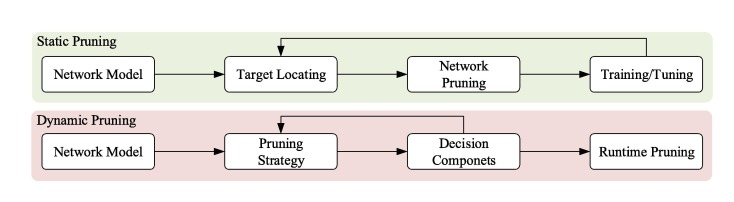
\includegraphics[width=0.75\linewidth]{images/dynamic pruning.jpg}
  \caption[Static pruning - dynamic pruning]{Static pruning - dynamic pruning. Nguồn \cite{45_LIANG2021370}}
  \label{fig:dyn_sta}
\end{figure}
Dựa trên thời điểm (Hình \ref{fig:dyn_sta}), cắt tỉa tĩnh (static pruning) được thực hiện ngoại tuyến trước thời gian runtime. Trong phương pháp này, các tham số bị loại bỏ và phương pháp cắt tỉa được lựa chọn dựa trên một tiêu chí nhất định, sau đó mô hình có thể tinh chỉnh lại để phục hồi độ chính xác, và cấu trúc mạng sau khi cắt tỉa được giữ cố định trong giai đoạn suy luận. Ngược lại, cắt tỉa động được thực hiện trong thời gian runtime, trong đó mô hình sử dụng các cơ chế ra quyết định (ví dụ như kết nối bổ trợ hoặc mạng quyết định bổ trợ) để xác định các thành phần nào sẽ được kích hoạt hoặc bỏ qua tùy theo từng đầu vào cụ thể. Cách tiếp cận này cho phép mô hình thích ứng linh hoạt với dữ liệu, tuy nhiên đồng thời cũng làm phát sinh chi phí tính toán bổ sung trong quá trình suy luận.

Dựa trên tiêu chí lựa chọn tham số để loại bỏ, các phương pháp cắt tỉa có thể được chia thành hai nhóm chính: magnitude-based pruning và penalty-based pruning. Trong đó, các phương pháp magnitude-based dựa trên giả định rằng các trọng số có độ lớn tuyệt đối cao đóng vai trò quan trọng hơn, trong khi các trọng số có giá trị nhỏ có thể bị loại bỏ mà không ảnh hưởng đáng kể đến hiệu suất mô hình. Cách tiếp cận này thường xác định và loại bỏ các trọng số hoặc đặc trưng dư thừa tại mức kernel hoặc activation map dựa trên một ngưỡng (threshold) định trước. Ngoài phương pháp ngưỡng đơn giản, một số kỹ thuật nâng cao còn sử dụng thông tin đạo hàm bậc hai của hàm mất mát như ma trận Hessian, hoặc các chuẩn $l_1$ và $l_2$ áp dụng trên từng trọng số hoặc nhóm trọng số để đánh giá mức độ quan trọng. Tổng quát, chuẩn $l_p$ của một vector $x\in R^n$ được định nghĩa như sau:
\begin{equation}
    \lVert x \rVert_p = (\sum\limits_{i=1}^n|x_i|^p)^{\frac{1}{p}}
\end{equation}.Ngược lại, penalty-based pruning tác động trực tiếp vào quá trình huấn luyện thông qua việc sửa đổi hàm mất mát hoặc bổ sung các ràng buộc nhằm khuyến khích tính thưa của mô hình. Cụ thể, một hàm phạt được thêm vào trong quá trình tối ưu để ép các trọng số kém quan trọng tiến dần về giá trị không hoặc gần bằng không. Sau khi huấn luyện hoàn tất, các trọng số này sẽ được loại bỏ khỏi mạng. Các kỹ thuật phổ biến trong nhóm này bao gồm weight decay (tương ứng với regularization chuẩn $l_2$), và các biến thể của LASSO. Phương pháp LASSO (Least Absolute Shrinkage and Selection Operator) có mục tiêu làm giảm độ lớn của trọng số, đưa nhiều trọng số tiến về giá trị 0, qua đó thúc đẩy tính thưa của mô hình. Bài toán tối ưu của LASSO có thể được biểu diễn như sau:
\begin{equation}
\begin{aligned}
& \text{arg}\min\limits_{\alpha,\beta}&\left\{\sum\limits_{i=1}^N(y_i-a-\sum\limits_{j=1}^p\beta_jx_{ij})^2\right\} \\
& \text{subject to} & \sum\limits_j^p|\beta_j| \leq t \\
&&\frac{\sum_ix_{ij}}{N}=0\\
&&\frac{\sum_ix_{ij}^2}{N}=1
\end{aligned}
\end{equation}
Trong đó, $x$, $y$ lần lượt là đầu vào và đầu ra, $\beta$ là vector trọng số, $t$ là tham số điều khiển mức độ thưa của mô hình. Ngoài hai hướng tiếp cận trên, một số phương pháp cắt tỉa còn khai thác tính dư thừa và trùng lặp trong không gian tham số, chẳng hạn như loại bỏ các bộ trọng số hoặc các kênh có mức độ tương đồng cao.
\begin{figure}[ht]
  \centering
  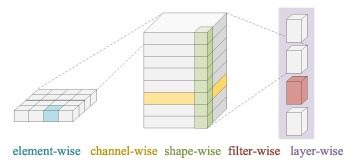
\includegraphics[width=0.5\linewidth]{images/elementwise.jpg}
  \caption[Phân loại cắt tỉa dựa trên mức độ chi tiết]{Phân loại cắt tỉa dựa trên mức độ chi tiết. Nguồn \cite{45_LIANG2021370}}
  \label{fig:struct}
\end{figure}
Dựa trên cấu trúc và mức độ chi tiết của phần tử bị loại bỏ, các phương pháp cắt tỉa có thể được phân thành hai nhóm chính: cắt tỉa phi cấu trúc (unstructured pruning) và cắt tỉa có cấu trúc (structured pruning). Trong đó, unstructured pruning loại bỏ các trọng số hoặc kết nối riêng lẻ tại các vị trí bất kỳ trong mạng mà không tuân theo một ràng buộc hình học hay cấu trúc cụ thể. Nhờ tính linh hoạt này, phương pháp có thể đạt được mức độ thưa (sparsity) rất cao mà không gây ảnh hưởng đáng kể đến độ chính xác, qua đó giảm đáng kể số lượng tham số của mô hình. Tuy nhiên, hệ quả là các ma trận trọng số sau khi cắt tỉa không có cấu trúc, gây khó khăn cho việc khai thác hiệu quả trên các phần cứng và thư viện tính toán tiêu chuẩn trừ khi có hỗ trợ chuyên biệt. 

Ngược lại, structured pruning loại bỏ các nhóm tham số có tổ chức, chẳng hạn như hàng, cột, kênh (channel-wise), hoặc bộ lọc (filter-wise) trong các lớp tích chập. Phương pháp này duy trì cấu trúc mạng đối xứng, tương thích tốt với các thư viện tính toán và phần cứng xử lý tập lệnh tiêu chuẩn, dẫn đến tốc độ thực thi nhanh hơn trong thực tế. Với mức ảnh hưởng cao, structured pruning cần được sử dụng cẩn thận và chính xác nhằm hạn chế mất thông tin nên mức độ thưa đạt được thường thấp hơn so với unstructured pruning. Tuy nhiên phương pháp này mang lại lợi ích đáng kể về tốc độ suy luận và khả năng triển khai thực tế, đặc biệt trên các thiết bị biên có tài nguyên hạn chế.
\begin{table}[htbp]
\centering
\small
\begin{tabular}{|p{2cm} |p{2.5cm}|p{2.5cm} |p{2.5cm}|p{2.5cm}|}
\hline
\textbf{Tiêu chí} & \textbf{Phân loại} & \textbf{Đặc điểm cốt lõi} & \textbf{Ưu điểm} & \textbf{Hạn chế} \\ 
\hline
\multirow{2}{=}{Thời điểm thực hiện} & \textbf{Static} & Thực hiện trước runtime & Đơn giản, cấu trúc mô hình cố định, dễ triển khai & Không thích ứng với dữ liệu mới \\ \cline{2-5}
 & \textbf{Dynamic} & Thực hiện tại runtime & Thích ứng cao với dữ liệu, duy trì hiệu suất tốt & Gây ra overhead tính toán \\ 
\hline
\multirow{2}{=}{Cấu trúc mạng} & \textbf{Unstructured} & Loại bỏ theo các trọng số riêng lẻ & Đạt tỷ lệ thưa cao nhất & Khó tăng tốc trên CPU/GPU thường \\ \cline{2-5}
 & \textbf{Structured} & Loại bỏ theo nhóm tham số & Tăng tốc phần cứng thực tế tốt & Độ thưa thấp và độ chính xác giảm nhanh khi nén cao. \\ 
\hline
\multirow{2}{=}{Tiêu chí lựa chọn} & \textbf{Magnitude-based} & Loại bỏ dựa trên giá trị tuyệt đối & Trực quan, chi phí tính toán xác định tham số thấp & Giả định độ lớn bằng tầm quan trọng không phải luôn đúng \\ \cline{2-5}
 & \textbf{Penalty-based} & Thêm ràng buộc để ép tham số tiến về 0 & Duy trì độ chính xác tốt & Quá trình huấn luyện phức tạp \\ 
\hline
\end{tabular}
\caption{Bảng so sánh các kỹ thuật cắt tỉa (Pruning)}
\label{tab:pruning_comparison}
\end{table}

\subsection{Lượng tử hóa}
\begin{figure}[ht]
  \centering
  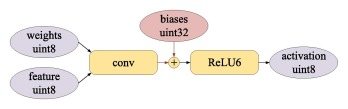
\includegraphics[width=0.75\linewidth]{images/1-s2.0-S0925231221010894-gr13.jpg}
  \caption[Integer Arithmetic-only Inference - một phương pháp lượng tử hóa thực tiễn]{Integer Arithmetic-only Inference - một phương pháp lượng tử hóa thực tiễn. Nguồn \cite{45_LIANG2021370}}
  \label{fig:quant-scheme}
\end{figure}
Lượng tử hóa (quantization) là quá trình xấp xỉ một tín hiệu liên tục bằng một tập hữu hạn các giá trị rời rạc, thường dưới dạng các số nguyên có độ chính xác thấp (numerical low-bit quantization). Trong bối cảnh nén mô hình học sâu, kỹ thuật này được sử dụng nhằm giảm băng thông bộ nhớ, dung lượng lưu trữ và mức tiêu thụ năng lượng, đồng thời tăng tốc độ xử lý. Cụ thể, các tham số ở dạng số thực dấu phẩy động 32-bit (FP32) được chuyển đổi sang các định dạng có độ chính xác thấp hơn, phổ biến nhất là số nguyên 8-bit (INT8), và trong một số trường hợp có thể xuống đến 4-bit, 2-bit hoặc 1-bit (ví dụ: mạng thần kinh nhị phân – BNN). 

Lượng tử hóa có thể được áp dụng lên các thành phần khác nhau của mạng như đặc trưng đầu vào (feature maps), trọng số (weights) và độ lệch (bias). Trong thực tế, bias thường chiếm tỷ lệ nhỏ trong tổng dung lượng mô hình và có độ nhạy cao đối với sai số, do đó thường được giữ ở độ chính xác cao. Tương tự, các lớp đầu vào và đầu ra của mạng cũng thường được giữ ở độ chính xác cao nhằm hạn chế suy giảm hiệu năng tổng thể. Trong quá trình suy luận, các phép toán như tích chập thường được thực hiện trực tiếp trên các giá trị đã lượng tử hóa và kết quả trung gian được tích lũy ở độ chính xác cao hơn. Sau đó, kết quả này được tái lượng tử hóa (requantization) về miền độ chính xác thấp để làm đầu vào cho lớp tiếp theo mà không cần trực tiếp dequantization kết quả đầu ra của lớp. Các hàm kích hoạt có thể được áp dụng trực tiếp trên đầu ra lượng tử, sau bước requantization hoặc đầu ra chính xác cao.

Về mặt toán học, lượng tử hóa có thể được biểu diễn tổng quát như một hàm ánh xạ giá trị thực $X_r$ sang giá trị lượng tử $X_q$ thông qua một hệ số tỉ lệ (scale - s) và một điểm không (zero-point - z) như sau:
\begin{equation}
    X_q = f(s\times g(X_r)+z)
\end{equation}
Trong đó $g(.) = clamp(x,\alpha,\beta) = \max(\min(x,\beta),\alpha)$ là hàm clamp giới hạn giá trị x trong khoảng $[\alpha,\beta]$, và hàm $f(⋅)$ là hàm round thực hiện làm tròn về biểu diễn lượng tử hóa gần nhất. Các phương pháp lượng tử hóa có thể được phân loại theo nhiều tiêu chí khác nhau, bao gồm: thời điểm áp dụng, cách nhóm đối tượng lượng tử hóa, cách ánh xạ dải giá trị và  độ rộng bit (bit-width). 
\begin{figure*}[ht]
    \centering
    \begin{subfigure}[t]{0.45\textwidth}
        \centering
        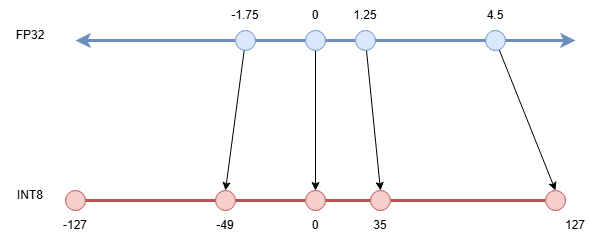
\includegraphics[width=\linewidth]{images/Quantization-max-abs.drawio.png}
        \caption{Lượng tử hóa đối xứng max-abs}
        \label{fig:syn_quant}
    \end{subfigure}%
    ~
    \begin{subfigure}[t]{0.45\textwidth}
        \centering
        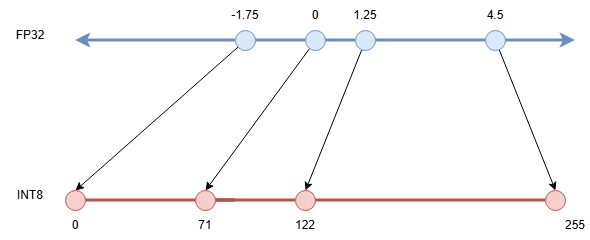
\includegraphics[width=\linewidth]{images/Quantization-min-max.drawio.png}
        \caption{Lượng tử hóa bất đối xứng min-max}
        \label{fig:asyn-quant}
    \end{subfigure}
    \caption{Các phương pháp lượng tử hóa từ FP32 sang INT8}
\end{figure*}

Dựa trên cách ánh xạ dải giá trị, các phương pháp lượng tử hóa có thể được chia thành ánh xạ đối xứng (symmetric quantization) và ánh xạ bất đối xứng (asymmetric quantization), tùy thuộc vào việc điểm không (zero-point) có bằng 0 hay không. Trong đó, ánh xạ đối xứng sử dụng z=0 và dải giá trị được phân bố đối xứng quanh gốc tọa độ. Cách tiếp cận này giúp đơn giản hóa phép toán trong quá trình suy luận, đặc biệt là trong các phép tích chập, do không cần xử lý thêm các thành phần bù (offset), từ đó giảm chi phí tính toán. Tuy nhiên, nhược điểm của ánh xạ đối xứng là khả năng biểu diễn kém hiệu quả hơn trong trường hợp dữ liệu không phân bố đối xứng quanh 0. Điều này đặc biệt rõ rệt đối với các đặc trưng sau hàm kích hoạt ReLU, khi toàn bộ giá trị nằm trên nửa trục dương, dẫn đến việc một nửa miền giá trị lượng tử không được sử dụng, làm giảm dynamic range hiệu dụng. Trong khi đó, ánh xạ bất đối xứng bảo toàn được sự linh hoạt trên miền lượng tử. Tuy nhiên, trong thực tế, sự khác biệt về độ chính xác giữa hai phương pháp là không đáng kể\cite{wang_2025_model}.

Dựa trên độ mịn (granularity), tức là phạm vi các tham số chia sẻ cùng một bộ tham số lượng tử hóa, các phương pháp lượng tử hóa có thể được chia thành hai dạng chính: per-layer và per-channel. Trong đó, per-layer quantization (lượng tử hóa theo lớp) sử dụng chung một bộ hệ số cho toàn bộ trọng số hoặc kích hoạt trong một lớp. Phương pháp này có ưu điểm là đơn giản, dễ triển khai và tiết kiệm bộ nhớ, tuy nhiên có thể dẫn đến sai số lượng tử hóa lớn hơn, đặc biệt khi phân phối dữ liệu không đồng nhất giữa các kênh hoặc chiều. Ngược lại, per-channel quantization (lượng tử hóa theo kênh) gán bộ tham số lượng tử hóa riêng cho từng kênh. Ưu điểm của cách tiếp cận này là cải thiện độ ổn định số học và độ chính xác của mô hình nhờ vào việc giảm ảnh hưởng của các giá trị ngoại lai (outliers), vốn có thể làm suy giảm hiệu quả lượng tử hóa trong các phương pháp thô hơn. Ngoài ra còn có per-block quantization (lượng tử hóa theo khối) cung cấp mức độ kiểm soát chi tiết hơn bằng cách chia tensor thành các khối nhỏ, mỗi khối được gán một bộ tham số lượng tử hóa riêng. 

Dựa trên việc quá trình lượng tử hóa có tham gia vào giai đoạn huấn luyện hay không, các phương pháp có thể được chia thành hai nhóm chính: lượng tử hóa sau huấn luyện (Post-Training Quantization - PTQ) và huấn luyện nhận thức lượng tử hóa (Quantization-Aware Training - QAT). Đây là cách phân loại phổ biến nhất trong thực tế.

PTQ là kỹ thuật thực hiện lượng tử hóa sau khi quá trình huấn luyện mô hình đã hoàn tất. Trong phương pháp này, các trọng số được giữ cố định và được ánh xạ sang miền độ chính xác thấp dựa trên dải giá trị đã xác định trước. Đối với các đặc trưng kích hoạt (activations), do phân phối giá trị phụ thuộc vào dữ liệu đầu vào, một tập dữ liệu đại diện (representative dataset) thường được sử dụng để ước lượng các tham số lượng tử hóa thông qua quá trình calibration. Quá trình này có thể được phân thành hai dạng: static calibration, trong đó tham số lượng tử hóa được cố định sau khi ước lượng, và dynamic calibration, trong đó các tham số có thể được cập nhật trong thời gian chạy. PTQ có ưu điểm là đơn giản, triển khai nhanh và không yêu cầu huấn luyện lại, tuy nhiên thường dẫn đến suy giảm độ chính xác mạnh trên các mô hình nhỏ hoặc khi sử dụng độ rộng bit thấp.

Ngược lại, QAT tích hợp trực tiếp ảnh hưởng của sai số lượng tử vào quá trình huấn luyện hoặc tinh chỉnh mô hình. Cụ thể, các phép lượng tử giả (fake quantization) được chèn vào đồ thị tính toán nhằm mô phỏng các sai số làm tròn và giới hạn giá trị (clipping) trong khi vẫn duy trì biểu diễn số chính xác cao cho việc cập nhật trọng số. Nhờ đó, mô hình có thể duy trì độ chính xác gần tương đương với mô hình FP32 ban đầu, ngay cả khi sử dụng các mức lượng tử hóa thấp. Tuy nhiên, QAT yêu cầu quy trình huấn luyện phức tạp hơn, thời gian tính toán dài hơn và cần truy cập vào tập dữ liệu huấn luyện gốc.
\begin{table}[htbp]
\centering
\small
\begin{tabular}{|p{1.8cm} |p{2.2cm}|p{2.8cm} |p{2.8cm} |p{2.8cm}|}
\hline
\textbf{Tiêu chí} & \textbf{Phân loại} & \textbf{Đặc điểm cốt lõi} & \textbf{Ưu điểm} & \textbf{Nhược điểm} \\ 
\hline

\multirow{4}{=}{Tính đối xứng} & \textbf{Symmetric} & Dải giá trị thực được ánh xạ đối xứng qua gốc tọa độ & Tốc độ xử lý nhanh & Có thể gây lãng phí dải động và tăng lỗi lượng tử nếu dữ liệu phân bố lệch một phía \\ \cline{2-5}
 & \textbf{Asymmetric} & Sử dụng điểm không ($z$) khác 0 & Duy trì độ chính xác cao cho dữ liệu không đều & Tăng chi phí tính toán \\ 
\hline

\multirow{4}{=}{Độ mịn} & \textbf{Per-layer} & Một bộ tham số duy nhất trong một lớp & Triển khai đơn giản, tiết kiệm bộ nhớ cho việc lưu trữ tham số lượng tử & Gây lỗi lượng tử lớn nếu phân bố dữ liệu khác biệt cao \\ \cline{2-5}
 & \textbf{Per-channel} & Mỗi kênh đầu ra có một bộ tham số riêng biệt & Độ chính xác cao & Phức tạp trong triển khai; tốn thêm bộ nhớ \\ 
\hline

\multirow{4}{=}{Phương thức thực hiện} & \textbf{PTQ} & Thực hiện trên mô hình đã hội tụ & Thực hiện cực kỳ nhanh; không đòi hỏi tài nguyên để huấn luyện lại mô hình & Sụt giảm độ chính xác mạnh trên các mô hình nhỏ hoặc mức nén bit cực thấp \\ \cline{2-5}
 & \textbf{QAT} & Tích hợp sai số lượng tử vào quá trình huấn luyện bằng cách mô phỏng & Duy trì độ chính xác tốt nhất; phục hồi độ chính xác của mô hình đã lượng tử hóa & Quy trình phức tạp; đòi hỏi thời gian huấn luyện lâu và cần tập dữ liệu đầy đủ \\ 
\hline
\end{tabular}
\caption{Bảng so sánh các kỹ thuật lượng tử hóa mạng thần kinh  (Quantization)}
\label{tab:quantization_comparison}
\end{table}